
\section{Introduction}

Building upon advances in multimodal understanding from models integrating vision and language~\citep{awadalla2023openflamingo,li2022blip,radford2021learning,an2024mc,luo2024llm}, Vision-Language-Action (VLA) models enable transformative embodied intelligence. These systems, such as OpenVLA~\citep{kim24openvla}, CogACT~\citep{li2024CogACT}, $pi_0$~\citep{black2024pi_0} and RT-2~\citep{brohan2023rt2visionlanguageactionmodelstransfer}, directly translate multimodal inputs into executable actions, successfully tackling complex robotic manipulation and reasoning tasks using large-scale datasets~\citep{fang2024rh20t,o2024open}. Many cutting-edge VLAs couple a Vision-Language Model (VLM) for scene and instruction parsing with a diffusion model to handle multi-modal action distribution~\citep{li2024CogACT,wen2024diffusion,wen2025dexvla,wen2024tinyvla}. However, the significant computational and memory overheads of these Diffusion-based VLA architectures during the inference time pose critical barriers to their practical deployment, particularly for real-time interaction on resource-constrained robotic platforms.

Diffusion-based VLA architectures typically comprise a vision encoder to extract features, a large language model (LLM)~\citep{touvron2023llama,floridi2020gpt,openai2024gpt4technicalreport,liu2019robertarobustlyoptimizedbert,wang2025data} core for multimodal reasoning, and a diffusion-based action decoder to predicts the final actions through multiple denoising steps. While this modular design underpins their powerful capabilities, it inherently results in substantial computational and memory overhead. Our findings (Table~\ref{table:vla_pruner_comparison}) indicate that the language module and the iterative diffusion head are primary contributors to overall latency and computational load. Furthermore, as illustrated in Figure~\ref{fig:bottleneck} (a), while visual token pruning initially reduces inference time in computation-bound scenarios, its efficacy quickly diminishes as the system becomes memory-bound by the LLM.

Prior VLA acceleration efforts have largely focused on isolated tweaks, delivering minimal overall gains. These fragmented approaches often fail because they ignore the integrated nature of VLA, where optimizing one module in isolation merely shifts bottlenecks. Gains are limited by unaddressed inefficiencies elsewhere, such as the memory demands of LLM or the computational intensity of action head. For example, methods like TinyVLA~\citep{wen2024tinyvla} and DeeR-VLA~\citep{DeeR-VLA} focus on specialized model architectures rather than broadly applicable inference acceleration frameworks for pre-trained VLAs. Other approaches, such as Mole-VLA~\citep{zhang2025mole}, tackle LLM layer redundancy but require costly retraining and overlook other pipeline stages. Similarly, VLA-Cache~\citep{xu2025vla} caches static visual tokens but provides limited speedup, constrained by the significant memory footprint of LLM and computational demands of the action head. Consequently, these existing approaches fall short of providing a truly holistic solution to navigate the complex landscape of VLA inefficiencies.



To develop a more effective acceleration strategy, we systematically analyze the inference characteristics and multifaceted redundancies within each VLA module. In many Diffusion-based VLAs, the diffusion action head operates as a separate module, guided by features extracted from the VLM. This separation may underutilize the full reasoning capacity of VLM for action generation, questioning the necessity of its entire scale.  As illustrated in Figure~\ref{fig:bottleneck} (b), the language module demonstrates shows considerable depth-wise representational redundancy with high inter-layer hidden state similarity.  The visual processing pathway exacerbates this issue by processing superfluous tokens, characterized by low task-relevance or high informational overlap due to visual similarity, which strains computational resources and intensifies the memory-bound condition of LLM. As shown in Figure~\ref{fig:bottleneck} (c), the iterative diffusion action head  displays significant temporal redundancy. The high similarity of its intermediate features across adjacent denoising steps implies extensive and near-static recomputations. 




\begin{table}[!t] 
  \caption{Module-wise inference characteristics of a baseline VLA model (CogACT, Left) compared to our proposed \mymethod{} (Right). \mymethod{} demonstrates significant improvements in overall inference speed and computational efficiency (FLOPs).}
  \label{table:vla_pruner_comparison} 
  \vspace{-10pt}
  \begin{minipage}[t]{0.49\linewidth} 
    \centering
    \label{table:latency_analysis_base}
    \resizebox{\linewidth}{!}{
      \begin{tabular}{r|ccc} 
        \toprule
         & Vision Module & Language Module & Action Module \\
        \hline
        \#Param (M) & 802.3 & 6738.9 & 89.0 \\
        Vision Token & 256 & 256 & - \\
        Denoising Steps & - & - & 10 \\
        Inference Time (ms) & 24.9 & 134.5 & 51.5 \\
        FLOPs (G) & 405.50 & 3726.55 & 57.96 \\
        \bottomrule
      \end{tabular}
    }
  \end{minipage}\hfill
  \begin{minipage}[t]{0.49\linewidth} 
    \centering
    \label{table:latency_analysis_ours}
    \resizebox{\linewidth}{!}{%
      \begin{tabular}{r|ccc} 
        \toprule
         & Vision Module & \textbf{Language Module} & \textbf{Action Module} \\
        \hline
        \#Param (M) & 802.3 & \textbf{3971.1} ($\downarrow$41\%) & 89.0 \\
        Vision Token & 256 & \textbf{56} ($\downarrow$78\%) & - \\
        Denoising Steps & - & - & \textbf{2} ($\downarrow$80\%) \\
        Inference Time (ms) & 24.9 & \textbf{58.9} ($\downarrow$56\%) & \textbf{26.2} ($\downarrow$49\%) \\
        FLOPs (G) & 405.50 & \textbf{792.58} ($\downarrow$78\%) & \textbf{11.72} ($\downarrow$80\%) \\
        \bottomrule
      \end{tabular}%
    }
  \end{minipage}
\end{table}


\begin{figure}[tb!]
    \centering
    \vspace{-10pt}
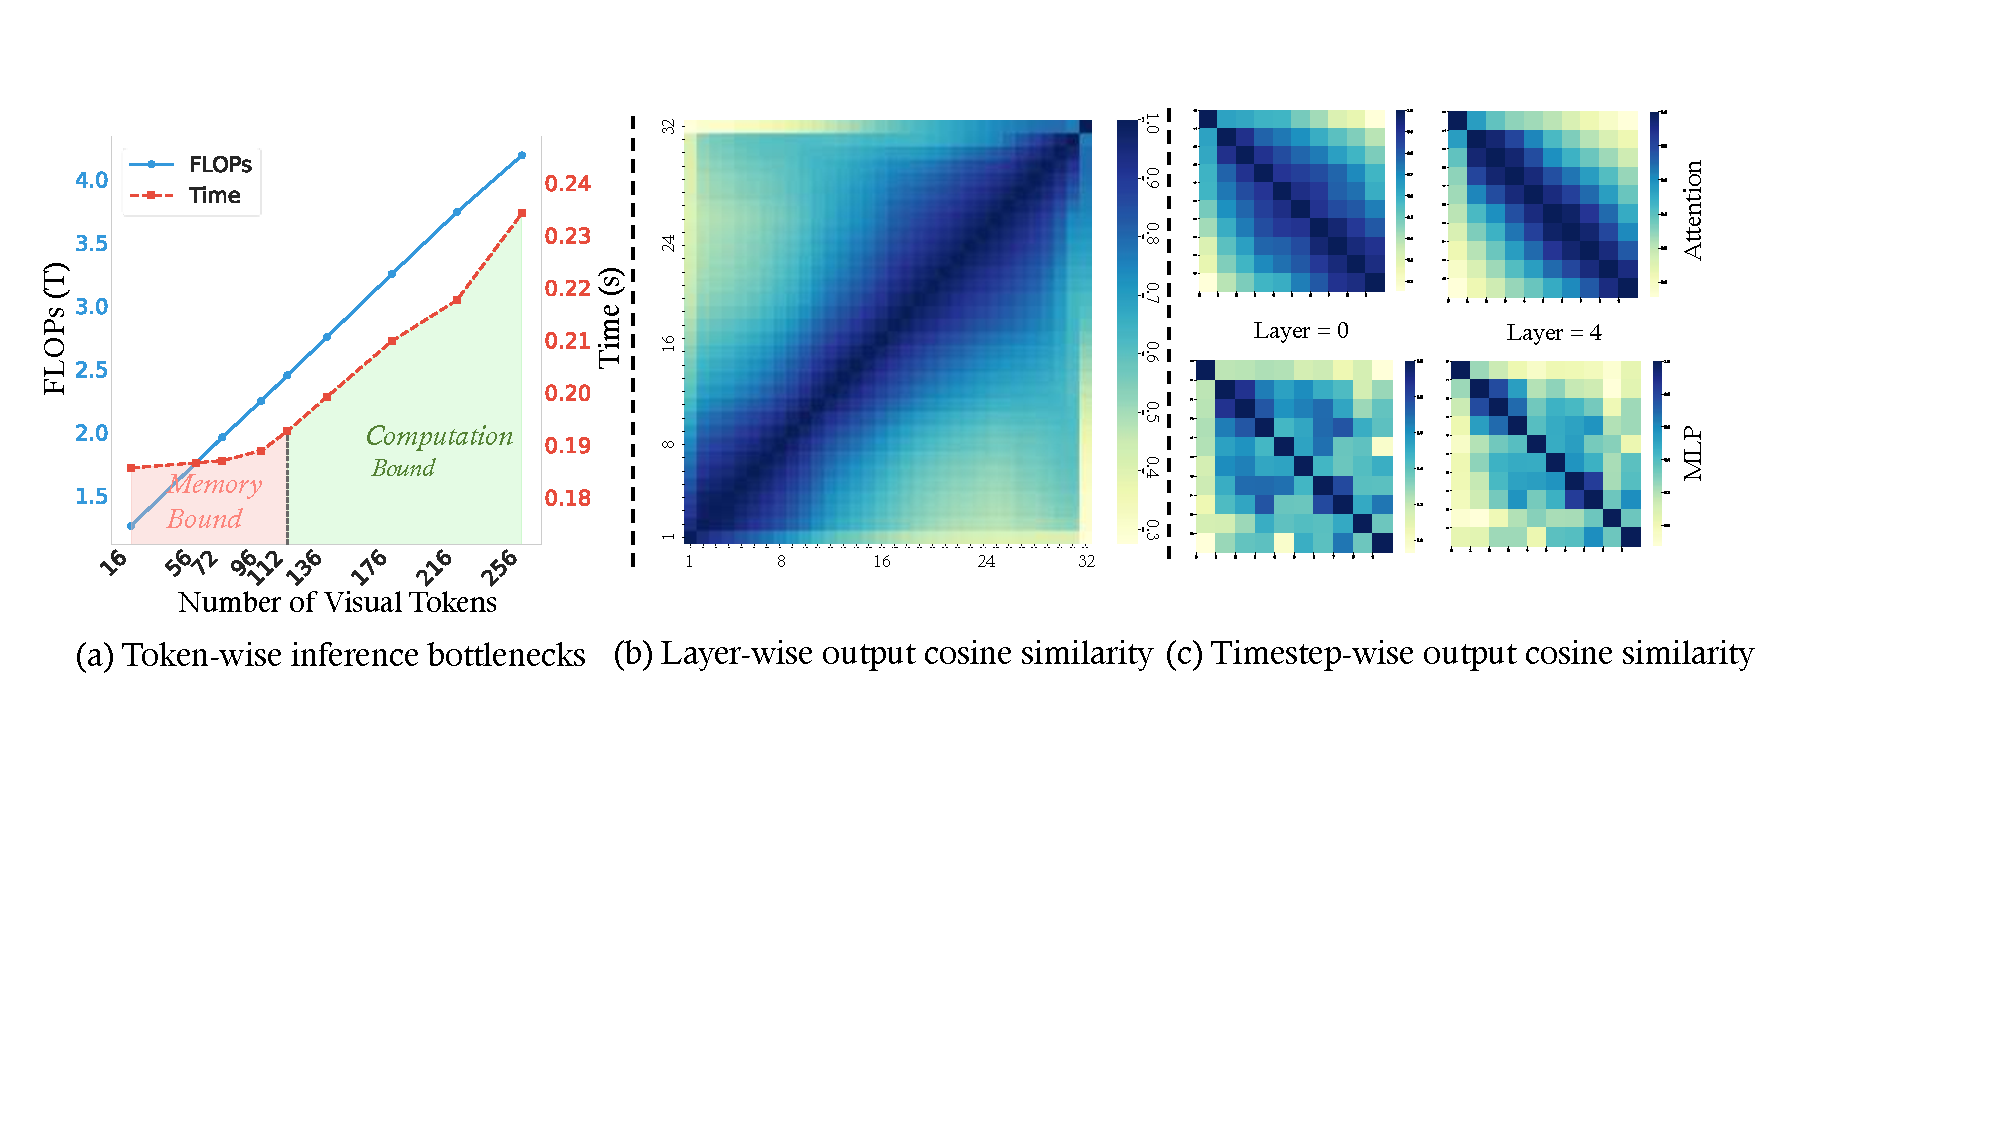
\includegraphics[width=0.99\linewidth]{figs/bottleneck.pdf}
    \vspace{-5pt}
    \caption{VLA inference bottleneck and redundancy analysis:
    \textbf{(a)}~Visual token pruning impact on FLOPs and inference time, revealing computation-bound and memory-bound regimes.
    \textbf{(b)}~High inter-layer cosine similarity of LLM hidden states, indicating depth-wise redundancy.
    \textbf{(c)}~Temporal cosine similarity of MLP/attention features in diffusion steps, showing computational redundancy. }
    \label{fig:bottleneck}
    \vspace{5pt}
\end{figure}


Motivated by this, we introduce \mymethod{}, a structured, training-free acceleration framework for Diffusion-based VLAs that systematically targets these issues. 
Using a similarity-derived importance metric to target the primary memory bottleneck of the language module and its observed depth-wise redundancy (Figure~\ref{fig:bottleneck} (b)), \mymethod{} employs a similarity-derived importance metric to prune functionally inconsequential layers, thus reducing the depth of the model and the demands for memory without retraining.
To manage the initial computational load from visual inputs before the memory of LLM limit is reached (Figure~\ref{fig:bottleneck} (a)), our visual token pruning strategy tackles both task-relevant and inherent image redundancies by first selecting critical task-aligned tokens, then augmenting this set to ensure representational diversity while maintaining high task relevance.
Lastly, \mymethod{} addresses temporal redundancy in the compute-intensive action generator (highlighted by high feature similarity across timesteps, Figure~\ref{fig:bottleneck} (c)) by caching and reusing intermediate attention and MLP outputs, thus curtailing redundant computations.
This synergistic, structured approach provides a more holistic alleviation of GPU compute and memory bottlenecks than isolated optimizations.




The main contributions of this work are summarized as follows:

\begin{enumerate}[leftmargin=10pt, topsep=0pt, itemsep=1pt, partopsep=1pt, parsep=1pt]
    \item We present a systematic analysis identifying critical computational and memory-bound bottlenecks, alongside multifaceted redundancies within contemporary Diffusion-based Vision-Language-Action (VLA) architectures, thereby motivating the need for structured acceleration.

    \item We propose \emph{\textbf{\mymethod{}}}, a novel training-free, structured inference acceleration framework that synergistically prunes redundant layers from the language module based on their informational impact and strategically selects a compact, task-focused subset of visual tokens by considering both VLA task relevance and inherent image feature diversity.

    \item Our framework further enhances efficiency by exploiting temporal redundancies in the diffusion-based action head, introducing a caching mechanism for intermediate attention and MLP computations during the iterative denoising process.

    \item We demonstrate the efficacy of \mymethod{} through extensive experiments on the CogACT in the SIMPLER environment~\citep{li2024evaluating}, achieving a $1.93\times$ inference speedup and reducing FLOPs to $28.9\%$, all while incurring a minimal accuracy degradation of only $0.6\%$. This will facilitate the application of large-scale VLAs on the resource-constrained robotics platforms in the real world. 
\end{enumerate}




